\documentclass[10pt,a4paper,headinclude,footinclude,hidelinks]{scrreprt} % KOMA-Script
\usepackage[italian]{babel}
\usepackage[utf8]{inputenc}
\usepackage[T1]{fontenc}
\usepackage{graphicx}
\usepackage{amsfonts}
\usepackage[]{../../classicthesis} % nochapters
\pagestyle{scrheadings}
\setcounter{tocdepth}{2}

\begin{document}
    \title{\rmfamily\normalfont\spacedallcaps{Modello relazionale}}
    \author{\spacedlowsmallcaps{Nicola Moretto (matr. 578258)}}
    \date{\today}
    
    \maketitle
    
    \begin{abstract}
        \noindent Il documento presenta il modello relazionale per l'integrazione dei nuovi criteri di classificazione nella piattaforma.
    \end{abstract}
    
	\begin{table}[ht]
	\centering
	\begin{tabular}{|c|c|l|}
	\hline
	\textsc{Versione} & \textsc{Data} & \textsc{Modifiche} \\ \hline
	0.1 & 2-10-2012 & Prima stesura del documento. \\ \hline
	\end{tabular}
	\caption{Registro delle modifiche}
	\label{tab:stage:wp:workload}
	\end{table}

	\tableofcontents

	%----------
	% CAPITOLO
	%----------
	\chapter{Schema relazionale}
	\label{ch:stage:er:schema}

	\begin{figure}[ht]
		\begin{center}
	    	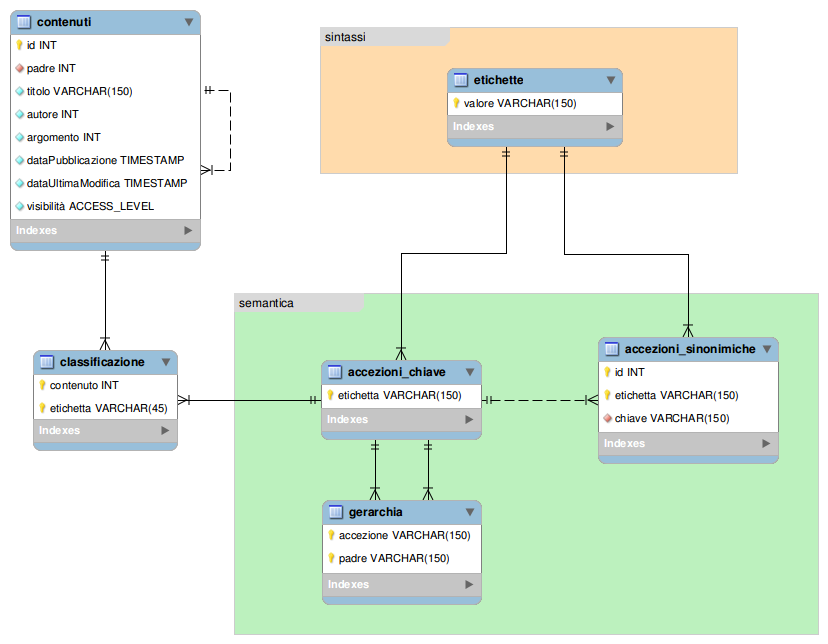
\includegraphics[width=14cm]{modello-er.png}
			\caption{Scherma relazionale del sistema di classificazione}
		\end{center}
	\end{figure}
 
	\section{Entit\`a}
	\section{Etichette}
	%Ciascuna etichetta rappresenta una parola o breve espressione in grado di identificare una o più entità del dominio. 
	\section{Accezioni}
	%Le accezioni rappresentano i possibili significati di un'etichetta, cui corrispondono altrettante entità riferibili.
	\subsection{Accezioni chiave}
	\subsection{Accezioni sinonimiche}

	%----------
	% CAPITOLO
	%----------
	\chapter{Operazioni}
	\label{ch:stage:er:operazioni}
	% ipotesi: rispetto del formato delle etichette (garantito in post-processing);
	% utilizzo di etichette o trigger;

	% SECTION
	\section{Etichette}
	\subsection{Ricerca di un'etichetta}
	\subsection{Ricerca delle accezioni di un'etichetta}
	\subsection{Inserimento di un'etichetta}
	\subsection{Eliminazione di un'etichetta}

	% SECTION
	\section{Accezioni}
	\subsection{Ricerca dell'accezione chiave}
	% Ricerca dell'accezione chiave associata all'accezione sinonimica di un etichetta.
	\subsection{Aggiunta di un'accezione}
	\subsubsection{Accezione chiave}
	\subsubsection{Accezione sinonimica}
	\subsection{Eliminazione di un'accezione}
	\subsubsection{Accezione chiave}
	\subsubsection{Accezione sinonimica}

	% SECTION
	\section{Entit\`a}
	\subsection{Ricerca dei figli}
	\subsection{Ricerca dei padri}
	\subsection{Ricerca dell'etichetta primaria}
	\subsection{Ricerca delle etichette secondarie}
	\subsection{Ricerca delle etichette}
	\subsection{Aggiungere un figlio}
	\subsection{Aggiungere un padre}
	%\subsection{Controllo di assenza cicli}

	% SECTION	
	\section{Contenuti}
	\subsection{Assegnazione di un'etichetta}
	\subsection{Ricerca delle etichette assegnate}
	\subsection{Ricerca di contenuti generici}
	\subsection{Ricerca di contenuti specifici}

\end{document}
